%\documentclass[]{beamer}
%\documentclass[handout]{beamer}
\documentclass[handout,draft]{beamer}

% Preambulo
% Paquetes para usar bien el idioma español
\usepackage[spanish,es-tabla]{babel}
\selectlanguage{spanish}
\usepackage[utf8]{inputenc}

% Paquetes para usar mejores imagenes
\usepackage{graphicx}

% Paquetes para links y tabla de contenidos en el PDF
\usepackage{hyperref}
\hypersetup{colorlinks=true,allcolors=blue}
%\usepackage{hypcap}

% Paquetes para mejores tablas
\usepackage{booktabs}

% Mejor matematica
\usepackage{amsmath}

% Fuentes de las imagenes
\usepackage[absolute,overlay]{textpos}

% Paquete captions
\usepackage[justification=centering,labelformat=empty,labelsep=none]{caption}

% Opciones para ticks
\usepackage{tikz}
\usetikzlibrary{shapes,arrows,positioning}

\tikzstyle{decision} = [diamond, draw, fill=blue!20, text width=4em, text badly centered, node distance=2cm, inner sep=0pt,on grid]
\tikzstyle{block} = [rectangle, draw, fill=blue!20, text width=8em, text centered, rounded corners, minimum height=2em,on grid]
\tikzstyle{line} = [draw, -latex]

% Citas bibliograficas
\usepackage[backend=biber]{biblatex}
\renewcommand{\footnotesize}{\tiny}
\addbibresource{biblio.bib}

% Mejoro las captions
\setbeamertemplate{caption}{\raggedright\insertcaption\par}

\setbeamertemplate{caption}{%
\begin{beamercolorbox}[wd=0.85\paperwidth, sep=.2ex]{block body}\insertcaption%
\end{beamercolorbox}%
}


% Sacar barra de navegacion
\setbeamertemplate{navigation symbols}{}%remove navigation symbols

% Transparencias en items
\setbeamercovered{transparent}

% Estilo de diapositivas
% \usetheme{Boadilla}
\usecolortheme{whale}
\usecolortheme{orchid}


\title{Herramientas de Teledetección Cuantitativa\\{\small Clase 5}}
\author{Francisco Nemi\~na}
\institute[Inst.]{
\includegraphics[height=1cm]{imagenes/logosopi.png}\phantom{pepe} 
\includegraphics[height=1cm]{imagenes/2mp.png}\phantom{pepe} 
\includegraphics[height=1cm]{imagenes/conae.png}}
\date{}
%\titlegraphic{
%\includegraphics[height=1cm]{IMAGENES/minplan.png}\phantom{1}
%
\includegraphics[height=1cm]{IMAGENES/conae.png}\phantom{1}
%
\includegraphics[height=1cm]{IMAGENES/sopi.png}}

\logo{
\includegraphics[height=0.7cm]{imagenes/sopi.png}}

\AtBeginSection[]
{
\begin{frame}
\frametitle{Esquema de presentaci\'on}
\tableofcontents[currentsection]
\end{frame}
}


\begin{document}
\begin{frame}
    \maketitle
\end{frame}

\section{Matem\'atica}
\subsection{Estad\'istica}
\begin{frame}{\subsecname}
  \begin{block}{Notaci\'on}
    Notamos a la media para la clase $\omega_i$ como $$m_i = \frac{1}{q_i-1} \sum_j^{q_i} x_j$$ donde $q_i$ es la cantidad de p\'ixeles de la clase.
  \end{block}\pause
  \begin{block}{Notaci\'on}
    La varianza como $$\sigma_i^2 = \frac{1}{q_i-1} \sum_j^{q_i} (x_j-m_i)^2$$ d\'onde los $x_j$ pertenecen a la clase $i$.
  \end{block}
\end{frame}
%--- Next Frame ---%

\begin{frame}{\subsecname}
  \begin{block}{Probabilidad condicional}
    Recordamos a la probabilidad condicional como $$p(x|\omega_i)$$ como la probabilidad de encontrar a un p\'ixel en el punto $x$ del espacio espectral dado que sabemos que pertenece a la clase $\omega_i$.
  \end{block}
\end{frame}
%--- Next Frame ---%

\begin{frame}{\subsecname}
  \begin{block}{Teorema de Bayes}
    $$p(\omega_i|x) = \frac{p(x|\omega_i) p(\omega_i)}{p(x)}$$
    Es decir, la probabilidad de que un p\'ixel pertenezca a la clase $\omega_i$ dado que se encuentra en el punto del espacio espectral $x$.
  \end{block}
\end{frame}
%--- Next Frame ---%

\begin{frame}{\subsecname}
  \begin{block}{Distribuci\'on de Gauss multidimensional}
    Si definimos a la matriz de covarianza como $$C_i = \frac{1}{q_i-1} \sum_j^{q_i} (x_j-m_i)(x_j-m_i)^T$$ podemos definir la distribuci\'on de Gauss en un espacio multidimensional como $$p(x|\omega_i) \sim \exp (\frac{-1}{2} (x-m_i)^T C_i^{-1} (x-m_i) )$$
  \end{block}
\end{frame}
%--- Next Frame ---%

\section{Clasificaci\'on supervisada}
\subsection{Idea}
\begin{frame}{Motivaci\'on}
  \begin{center}
      \resizebox{0.4 \linewidth}{!}{%
        \begin{tikzpicture}[node distance = 2cm, auto]
          \node[block]                                (init) {Firma Espectral};\pause
          \node[block, below= of init]                (resp) {Reflectancia Espectral Efectiva};
          \path[line] (init) --          (resp);
          \pause
          \node[block, below= of resp]             (ques) {Categor\'ias};
          \path[line] (resp) --          (ques);\pause
        \end{tikzpicture}%
      }%
    \end{center}
\end{frame}
%--- Next Frame ---%

\begin{frame}{\subsecname}
  \begin{alertblock}{Importante}
    Ahora tenemos que definir apriori cuales son las clases que queremos y como encontrarlas.
  \end{alertblock}
\end{frame}
%--- Next Frame ---%

\begin{frame}{\subsecname}
  \begin{figure}
  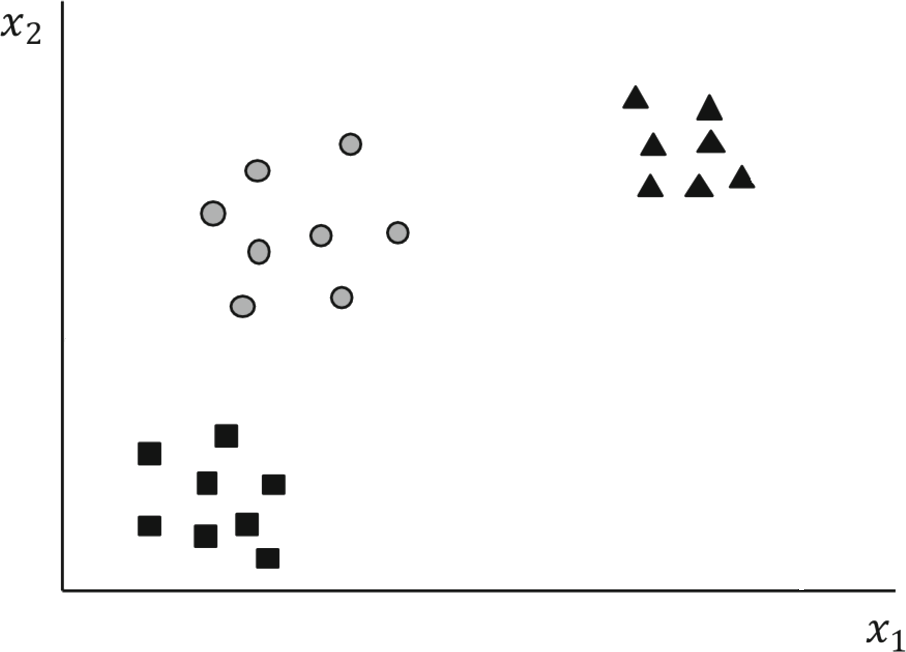
\includegraphics[width=0.6\textwidth]{imagenes/vector-3.png}
  \caption{Espacio vectorial.\footfullcite{richards2013remote}}
  \end{figure}
\end{frame}
%--- Next Frame ---%

\begin{frame}{\subsecname}
  \begin{figure}
  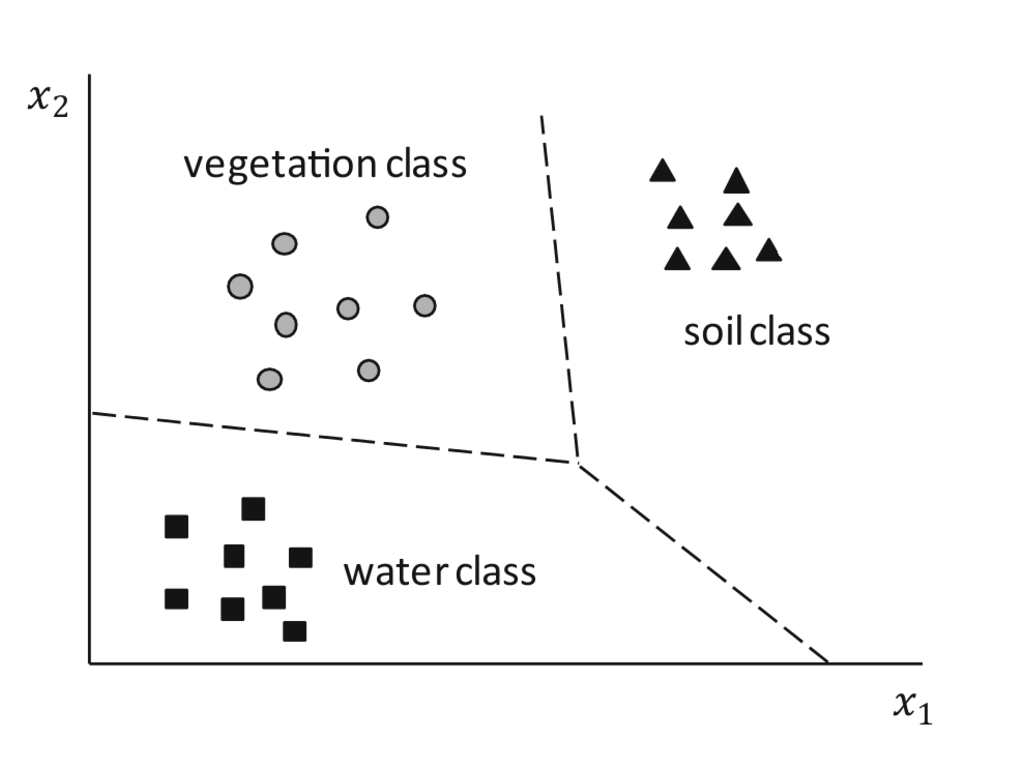
\includegraphics[width=0.6\textwidth]{imagenes/vector-2.png}
  \caption{Clasificaci\'on del espacio vectorial a partir de clases de entrenamiento.\footfullcite{richards2013remote}}
  \end{figure}
\end{frame}

\begin{frame}{\subsecname}
  \begin{block}{Esquema general}
    \begin{enumerate}[<+>]
      \item Decidir cuales son las clases de intere\'es.
      \item Elegir p\'ixeles conocidos y representativos para cada clase a utilizar como \'areas de entrenamiento.
      \item Estimar los par\'ametros del m\'etodo de clasificaci\'on.
      \item Usar el clasificador para clasificar los pixeles.
      \item Producir mapas tem\'aticos para extraer informaci\'on.
      \item Corroborar la precisi\'on de la clasificaci\'on con datos de campo
    \end{enumerate}
  \end{block}
\end{frame}
%--- Next Frame ---%

%--- Next Frame ---%
\subsection{M\'etodos}
\begin{frame}{\subsecname}
  \begin{block}{Generales}
    \begin{itemize}
      \item<.> Paralelep\'ipedos
      \item<.> Distancia m\'inima
      \item<1> M\'axima verosimilitud
      \item<.> \'Angulo espectral
    \end{itemize}
  \end{block}
\end{frame}
%--- Next Frame ---%

\subsection{M\'axima verosimilitud}

\begin{frame}{\subsecname}
  \begin{block}{Clasificador Bayesiano}
    Si conocemos las probabilidades condicionales $p(\omega_i|x)$ entonces un p\'ixel $x$ pertenece a la clase $\omega_i$ si $$p(\omega_i|x)>p(\omega_j|x)$$ si $i \neq j$.
  \end{block}
  \pause
  \begin{alertblock}{Problema}
    No conocemos $p(\omega_i|x)$.
  \end{alertblock}
\end{frame}
%--- Next Frame ---%

\begin{frame}{\subsecname}
  \begin{block}{Soluci\'on}
    Usamos el teorema de Bayes y podemos escribir que un p\'ixel $x$ pertenece a la clase $\omega_i$ si $$p(x|\omega_i)p(\omega_i)>p(x|\omega_j)p(\omega_j)$$ si $i \neq j$.
  \end{block}
  \pause
  \begin{block}{Funci\'on discriminante}
    Si definimos $g_i(x) = \log (p(x|\omega_i)p(\omega_i))$ entonces lo anterior se convierte en $x$ pertenece a la clase $\omega_i$ si $$g_i(x)>g_j(x)$$ si $i \neq j$.
  \end{block}
\end{frame}
%--- Next Frame ---%

\begin{frame}{\subsecname}
  \begin{block}{Caso Gaussiano}
    Si suponemos que la distribuci\'on $p$ es normal y que, apriori la probabilidad de pertenecer a una clase es equiprobable, tenemos que
    $$g_i(x) = -\log |C_i| - (x-m_i)^T C_i^{-1} (x-m_i)$$.
  \end{block}
  \pause
  \begin{alertblock}{Observaciones:}
    Como la distribuci\'on de Gauss no se anula nunca, esto puede clasificar a lo largo de todo el espacio
  \end{alertblock}
\end{frame}
%--- Next Frame ---%

\begin{frame}{\subsecname}
  \begin{block}{Superficies de equiprobabilidad}
    Si buscamos la superficies de $$g_i = g_j$$ ese espacio queda dividido en distintos sectores donde es siempre mayor la probabilidad de pertenecer a una clase.
    \pause
    Son
    \begin{itemize}[<+>]
      \item Elipses
      \item Par\'abolas
      \item Hip\'erbolas
    \end{itemize}
  \end{block}
\end{frame}
%--- Next Frame ---%

\begin{frame}{\subsecname}
  \begin{figure}
  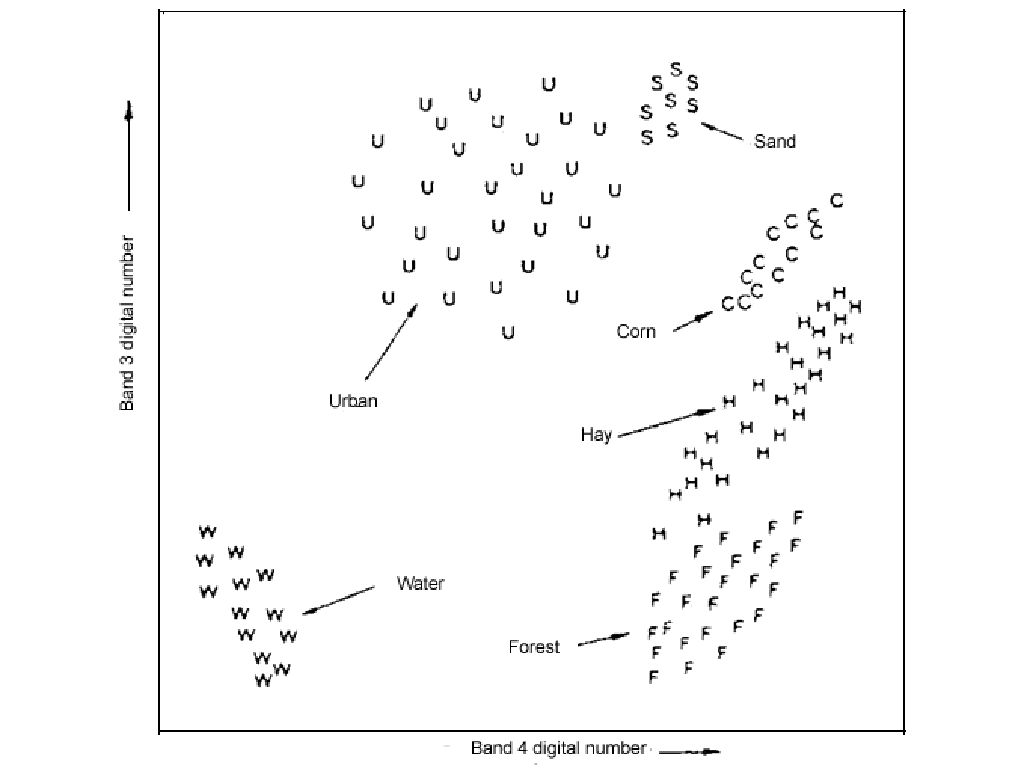
\includegraphics[width=0.6\textwidth]{imagenes/areas.png}
  \caption{Vista en el espacio vectorial.\footfullcite{clasif1}}
  \end{figure}
\end{frame}
%--- Next Frame ---%

\begin{frame}{\subsecname}
  \begin{figure}
  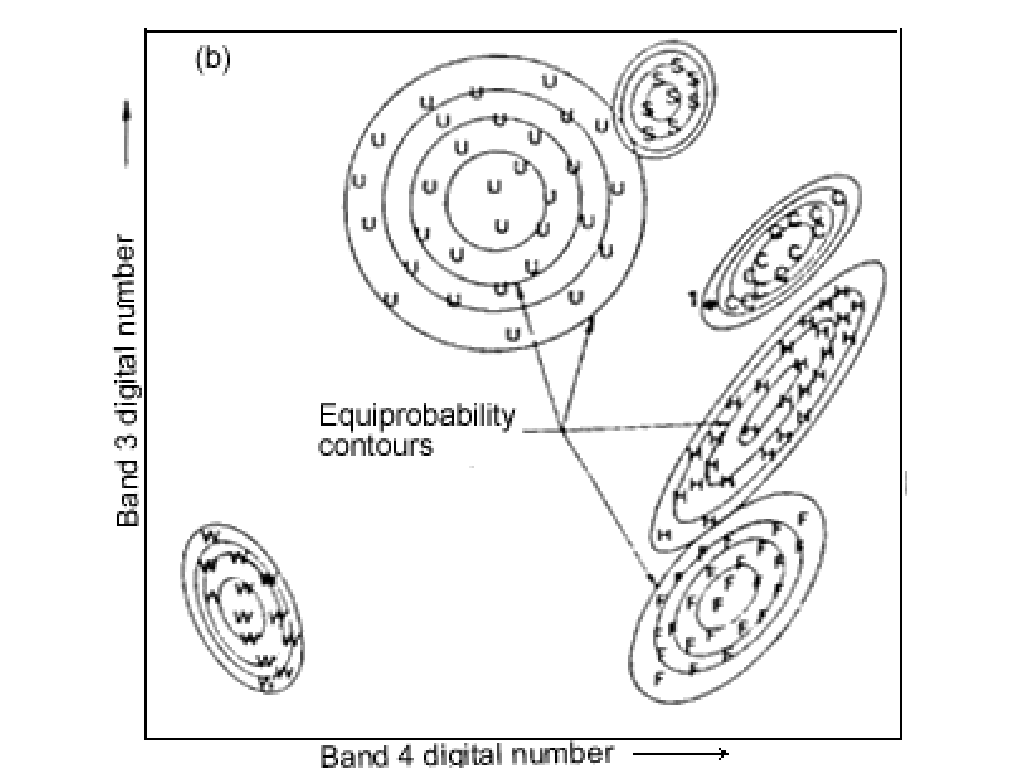
\includegraphics[width=0.6\textwidth]{imagenes/max.png}
  \caption{Vista en el espacio vectorial.\footfullcite{clasif1}}
  \end{figure}
\end{frame}
%--- Next Frame ---%

\begin{frame}{\subsecname}
  \begin{block}{N\'umero de p\'ixeles necesarios}
    Para estimar la matriz de covarianza se necesitan al menos $N(N+1)$ elementos. Es decir, al menos $N+1$ p\'ixeles.
  \end{block}
\end{frame}
%--- Next Frame ---%

\begin{frame}{\subsecname}
  \begin{figure}
  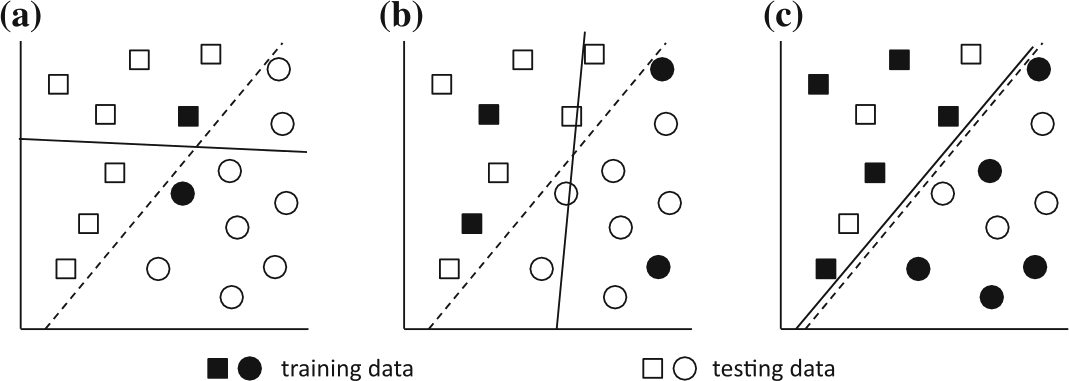
\includegraphics[width=0.8\textwidth]{imagenes/train.png}
  \caption{Clasificaci\'on supervisada incrementando el n\'umero de p\'ixeles de entrenamiento.\footfullcite{richards2013remote}}
  \end{figure}
\end{frame}
%--- Next Frame ---%

\begin{frame}{\subsecname}
  \begin{alertblock}{N\'umero de p\'ixeles necesarios}
    En la pr\'actica, se necesitan entre $10N$ y $100N$ p\'ixeles.
  \end{alertblock}
\end{frame}
%--- Next Frame ---%

\begin{frame}{\subsecname}
  \begin{figure}
  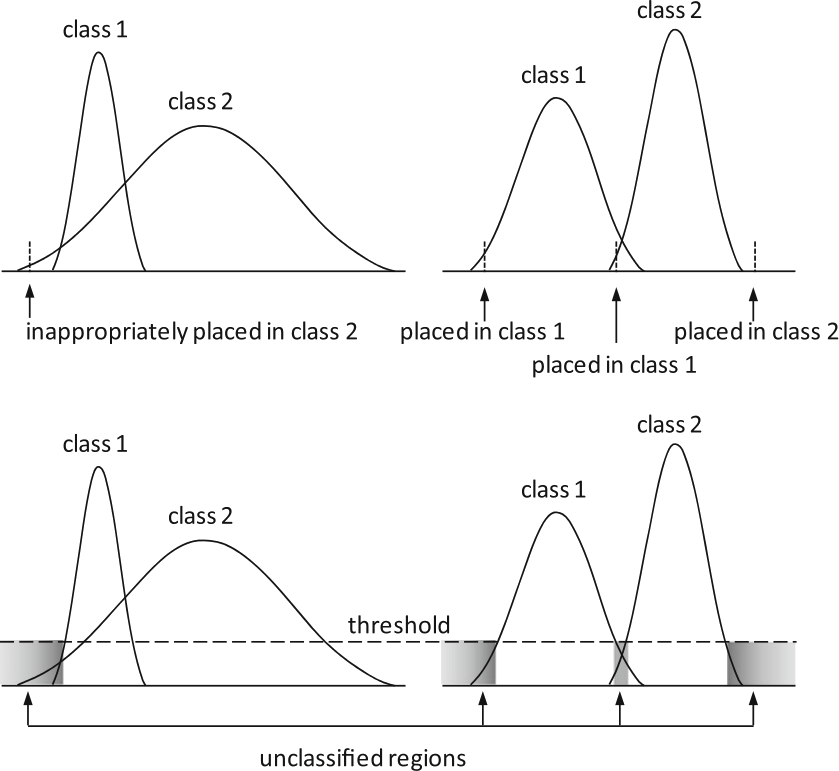
\includegraphics[width=0.6\textwidth]{imagenes/thresh.png}
  \caption{Problemas de clasificaci\'on y umbral.\footfullcite{richards2013remote}}
  \end{figure}
\end{frame}
%--- Next Frame ---%

\begin{frame}{\subsecname}
  \begin{figure}
  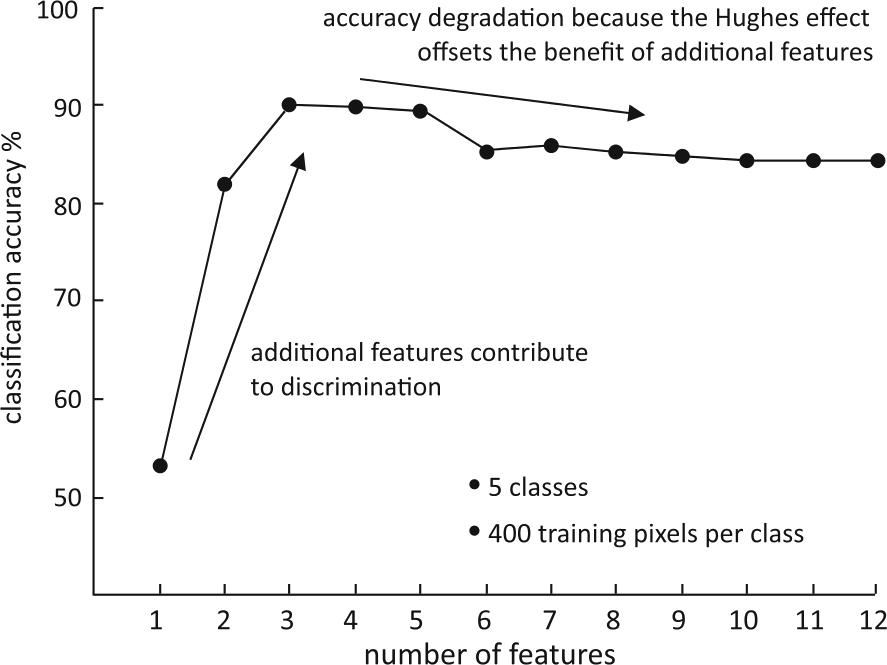
\includegraphics[width=0.8\textwidth]{imagenes/hughes.png}
  \caption{Otro problema, fen\'omeno de Hughes.\footfullcite{richards2013remote}}
  \end{figure}
\end{frame}
%--- Next Frame ---%

\begin{frame}{\subsecname}
  \begin{figure}
  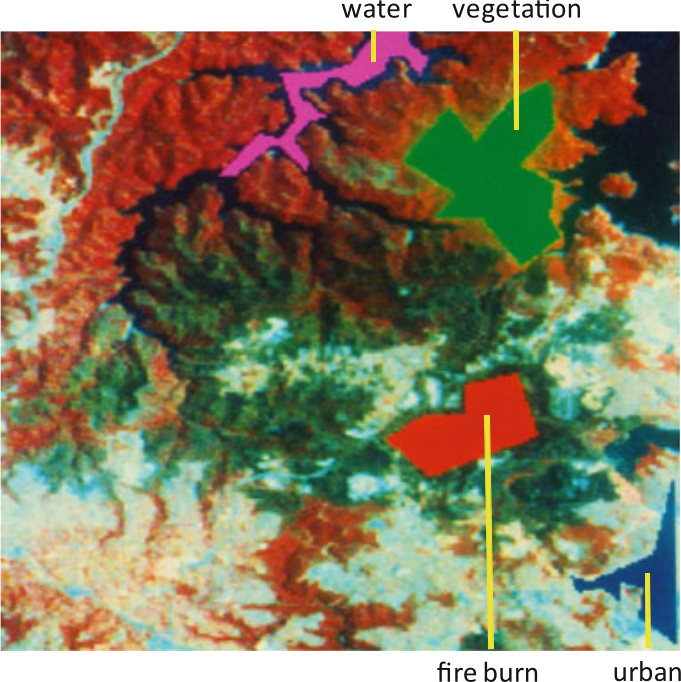
\includegraphics[width=0.6\textwidth]{imagenes/t_area.png}
  \caption{Imagen con \'areas de entrenamineto.\footfullcite{richards2013remote}}
  \end{figure}
\end{frame}
%--- Next Frame ---%

\begin{frame}{\subsecname}
  \begin{figure}
  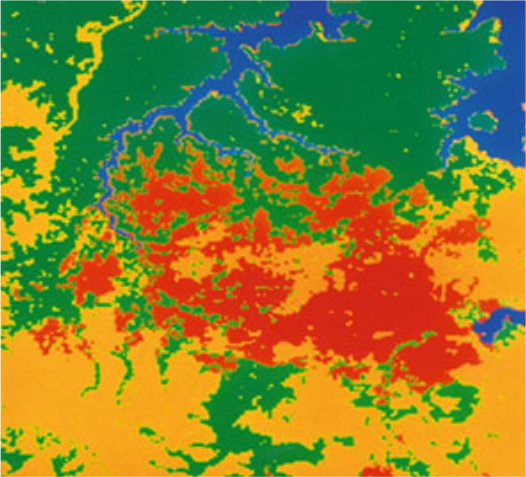
\includegraphics[width=0.6\textwidth]{imagenes/t_map.png}
  \caption{Imagen clasificada.\footfullcite{richards2013remote}}
  \end{figure}
\end{frame}
%--- Next Frame ---%

\subsection{Otros m\'etodos}
\begin{frame}{\subsecname}
  \begin{block}{Pocos p\'ixeles}
    Si contamos con pocos p\'ixeles de entrenamiento, podemos caer en otros metodos.
    \begin{itemize}
      \item<.> Paralelep\'ipedos
      \item<1> Distancia m\'inima
      \item<.> M\'axima verosimilitud
      \item<1> \'Angulo espectral
    \end{itemize}
  \end{block}
\end{frame}
%--- Next Frame ---%

\begin{frame}{\subsecname}
  \begin{block}{Distancia m\'inima}
    Si buscamos la superficies de $g_i = g_j$ con $g_i = 2 m_i x - m_i m_i$
    y me divide a mi espacio por hiperplanos.
  \end{block}
\end{frame}
%--- Next Frame ---%

\begin{frame}{\subsecname}
  \begin{figure}
  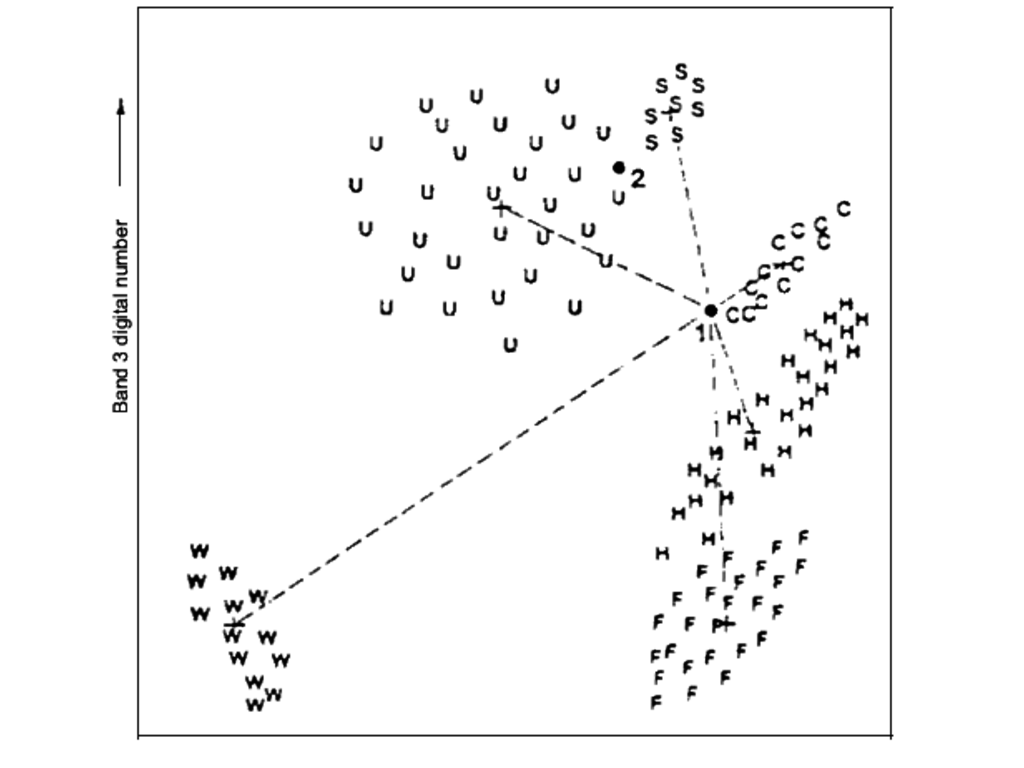
\includegraphics[width=0.6\textwidth]{imagenes/min.png}
  \caption{Vista en el espacio vectorial.\footfullcite{clasif1}}
  \end{figure}
\end{frame}
%--- Next Frame ---%

\begin{frame}{\subsecname}
  \begin{block}{Angulo espectral}
    Dividimos en este caso al espacio utilizando el \'angulo correspondiente a los p\'ixeles de entrenamiento.
  \end{block}
\end{frame}
%--- Next Frame ---%

\begin{frame}{\subsecname}
  \begin{figure}
  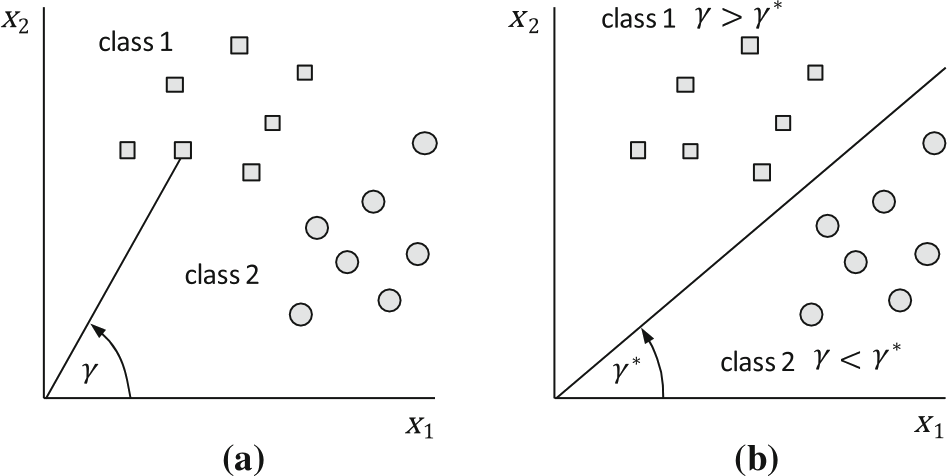
\includegraphics[width=0.6\textwidth]{imagenes/angle.png}
  \caption{Vista en el espacio vectorial.\footfullcite{richards2013remote}}
  \end{figure}
\end{frame}
%--- Next Frame ---%

\section{Pr\'actica}

\begin{frame}{\secname}
  \begin{exampleblock}{Actividades pr\'acticas de la cuarta clase}
    \begin{enumerate}[<+>]
      \item Abra las im\'agenes Landsat 8 y digitalice las coberturas de inter\'es.
      \item Clasifique la imagen utilizando un vector de entrenamiento por clase.
      \item Clasifique la imagen utilizando varios vectores de entrenamiento por clase.
      \item Utilizce la herramienta de estad\'isticas globales para estimar las \'areas correspondientes a cada uso y cobertura.
    \end{enumerate}
  \end{exampleblock}
\end{frame}
%--- Next Frame ---%

\end{document}
